\documentclass[12pt,a4paper]{article}
\usepackage[T2A]{fontenc}
\usepackage[utf8]{inputenc}
\usepackage[russian]{babel}
\usepackage{amsmath,amssymb,amsthm}
\usepackage{geometry}
\usepackage{hyperref}
\usepackage{microtype}
\usepackage{setspace}
\usepackage{caption}
\usepackage{graphicx}

\geometry{left=25mm, right=25mm, top=25mm, bottom=25mm}

\hypersetup{
  colorlinks=true,
  linkcolor=black,
  urlcolor=blue,
  pdfauthor={Тишковец Сергей},
  pdftitle={Отчёт по курсовой работе — Часть №4}
}

\begin{document}
\selectlanguage{russian}

\begin{titlepage}
  \begin{center}
    {Санкт-Петербургский политехнический университет Петра Великого\\
    Институт прикладной математики и механики\\[0.5em]
    \textbf{Высшая школа прикладной математики и вычислительной физики}}
  
    \vfill
  
    {\LARGE\bfseries Отчёт по курсовой работе\\ Часть №4\par}
    \vspace{1em}
    {\Large по дисциплине\\[0.3em] {\bfseries «Проект по математической статистике»}}
  
    \vfill
  
    \begin{flushright}
        Выполнил\\
        студент гр. 5030102/20202: Тишковец Сергей
    \end{flushright}
  
    \begin{flushright}
        Проверил\\
        Преподаватель: Заяц Олег Иванович
    \end{flushright}
  
    \vfill
    Санкт-Петербург\\
    2026
  \end{center}
\end{titlepage}

\setcounter{page}{2}
\newpage

\section*{Вычисление ОИСКО ядерной оценки методом Монте-Карло и оценка закона его распределения}

В четвёртой части курсовой работы проводится численное исследование точности ядерной оценки плотности равномерного распределения с помощью метода Монте-Карло, а также оценивается закон распределения величины ОИСКО.

Рассматривается равномерное распределение с плотностью:
\[
f_0(x) = 
\begin{cases}
\dfrac{1}{2\sqrt{3}}, & |x| \le \sqrt{3}, \\
0, & |x| > \sqrt{3}.
\end{cases}
\]

Ядерная оценка плотности с колокольным ядром имеет вид:
\[
\hat{f}_h(x) = \frac{1}{nh} \sum_{i=1}^n K\left( \frac{x - X_i}{h} \right),
\]
где \( K(u) = \frac{1}{\sqrt{2\pi}} \exp\left( -\frac{u^2}{2} \right) \), а параметр сглаживания \(\xi = h\).

\subsection*{1. Вычисление ОИСКО методом Монте-Карло (ММК)}

Процедура состоит из следующих шагов:

1. Генерируется \(N\) независимых выборок объёма \(n\) из распределения \(f_0(x)\).

2. Для каждой выборки и каждого фиксированного значения параметра \(\xi\) строится ядерная оценка \(\hat{f}(x)\).

3. Для каждой реализации численно вычисляется интегральная квадратичная ошибка (ОИСКО):
   \[
   \text{ISE}^{(k)}(\xi) = \int_{-\infty}^{\infty} \bigl(\hat{f}^{(k)}(x) - f_0(x)\bigr)^2 \, dx.
   \]
4. Оценка ОИСКО получается усреднением по всем \(N\) реализациям:
   \[
   \bar{\delta}_n(\xi) \approx \frac{1}{N} \sum_{k=1}^N \text{ISE}^{(k)}(\xi).
   \]

\subsection*{2. Оценка закона распределения величины ОИСКО}

Во второй части эксперимента фиксируется объём выборки \(n\) и оптимальное (или близкое к оптимальному) значение параметра \(\xi\). Затем генерируется большое количество \(N\) независимых выборок, для каждой из которых вычисляется значение \(\bar{\delta}_n^{(k)}(\xi)\).

Полученная выборка значений \(\{\bar{\delta}_n^{(k)}\}_{k=1}^N\) используется для построения эмпирической оценки закона распределения случайной величины ОИКО ядерной оценки. Для этого строятся гистограммы плотности при различных значениях \(N\) (число повторных реализаций).

Такой подход позволяет визуально оценить форму распределения ошибки ядерной оценки и понять, насколько устойчива оценка при данном объёме выборки.

\section*{Построение графиков}

\subsection*{График 1. Зависимость ОИСКО \(\bar{\delta}_n(\xi)\) (ММК)}

\begin{figure}[ht!]
    \centering
    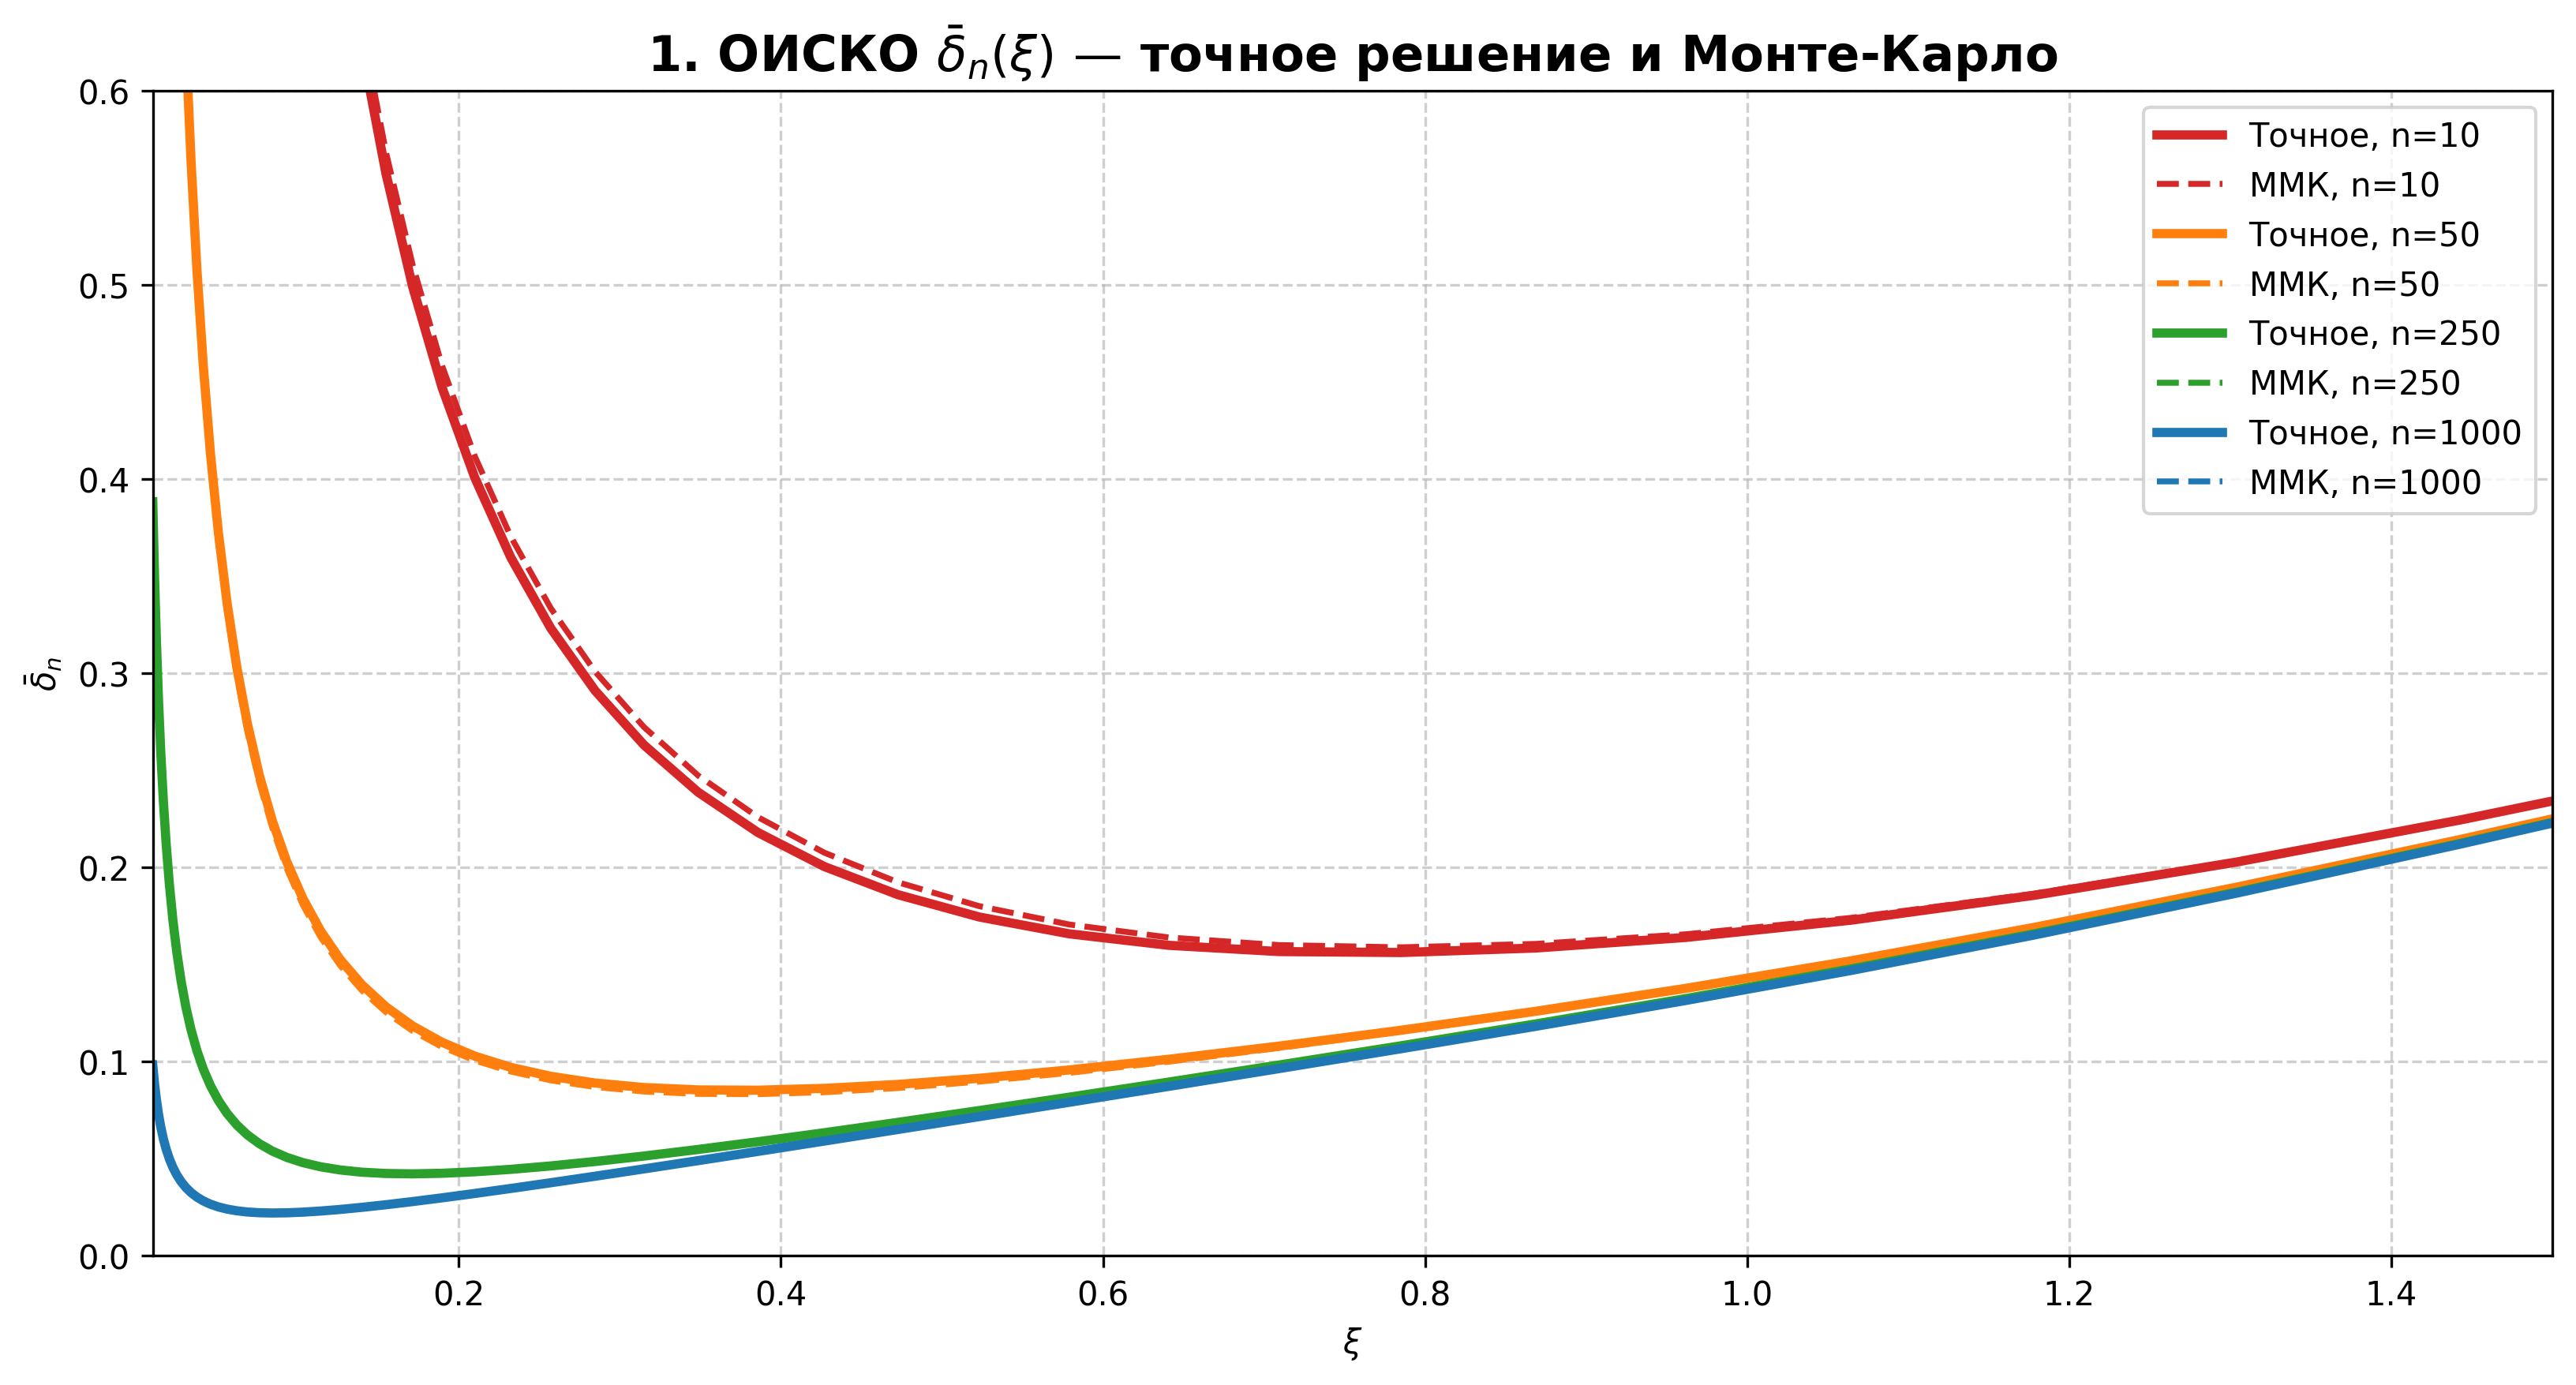
\includegraphics[width=0.85\textwidth]{figures/f12.png}
    \caption{Сравнение точного аналитического решения и оценки, полученной методом Монте-Карло, для различных объёмов выборки \(n\)}
    \label{fig:delta_xi_mmc}
\end{figure}

\subsection*{График 2. Зависимость \(\xi_{opt}\) от объёма выборки \(n\)}

\begin{figure}[ht!]
    \centering
    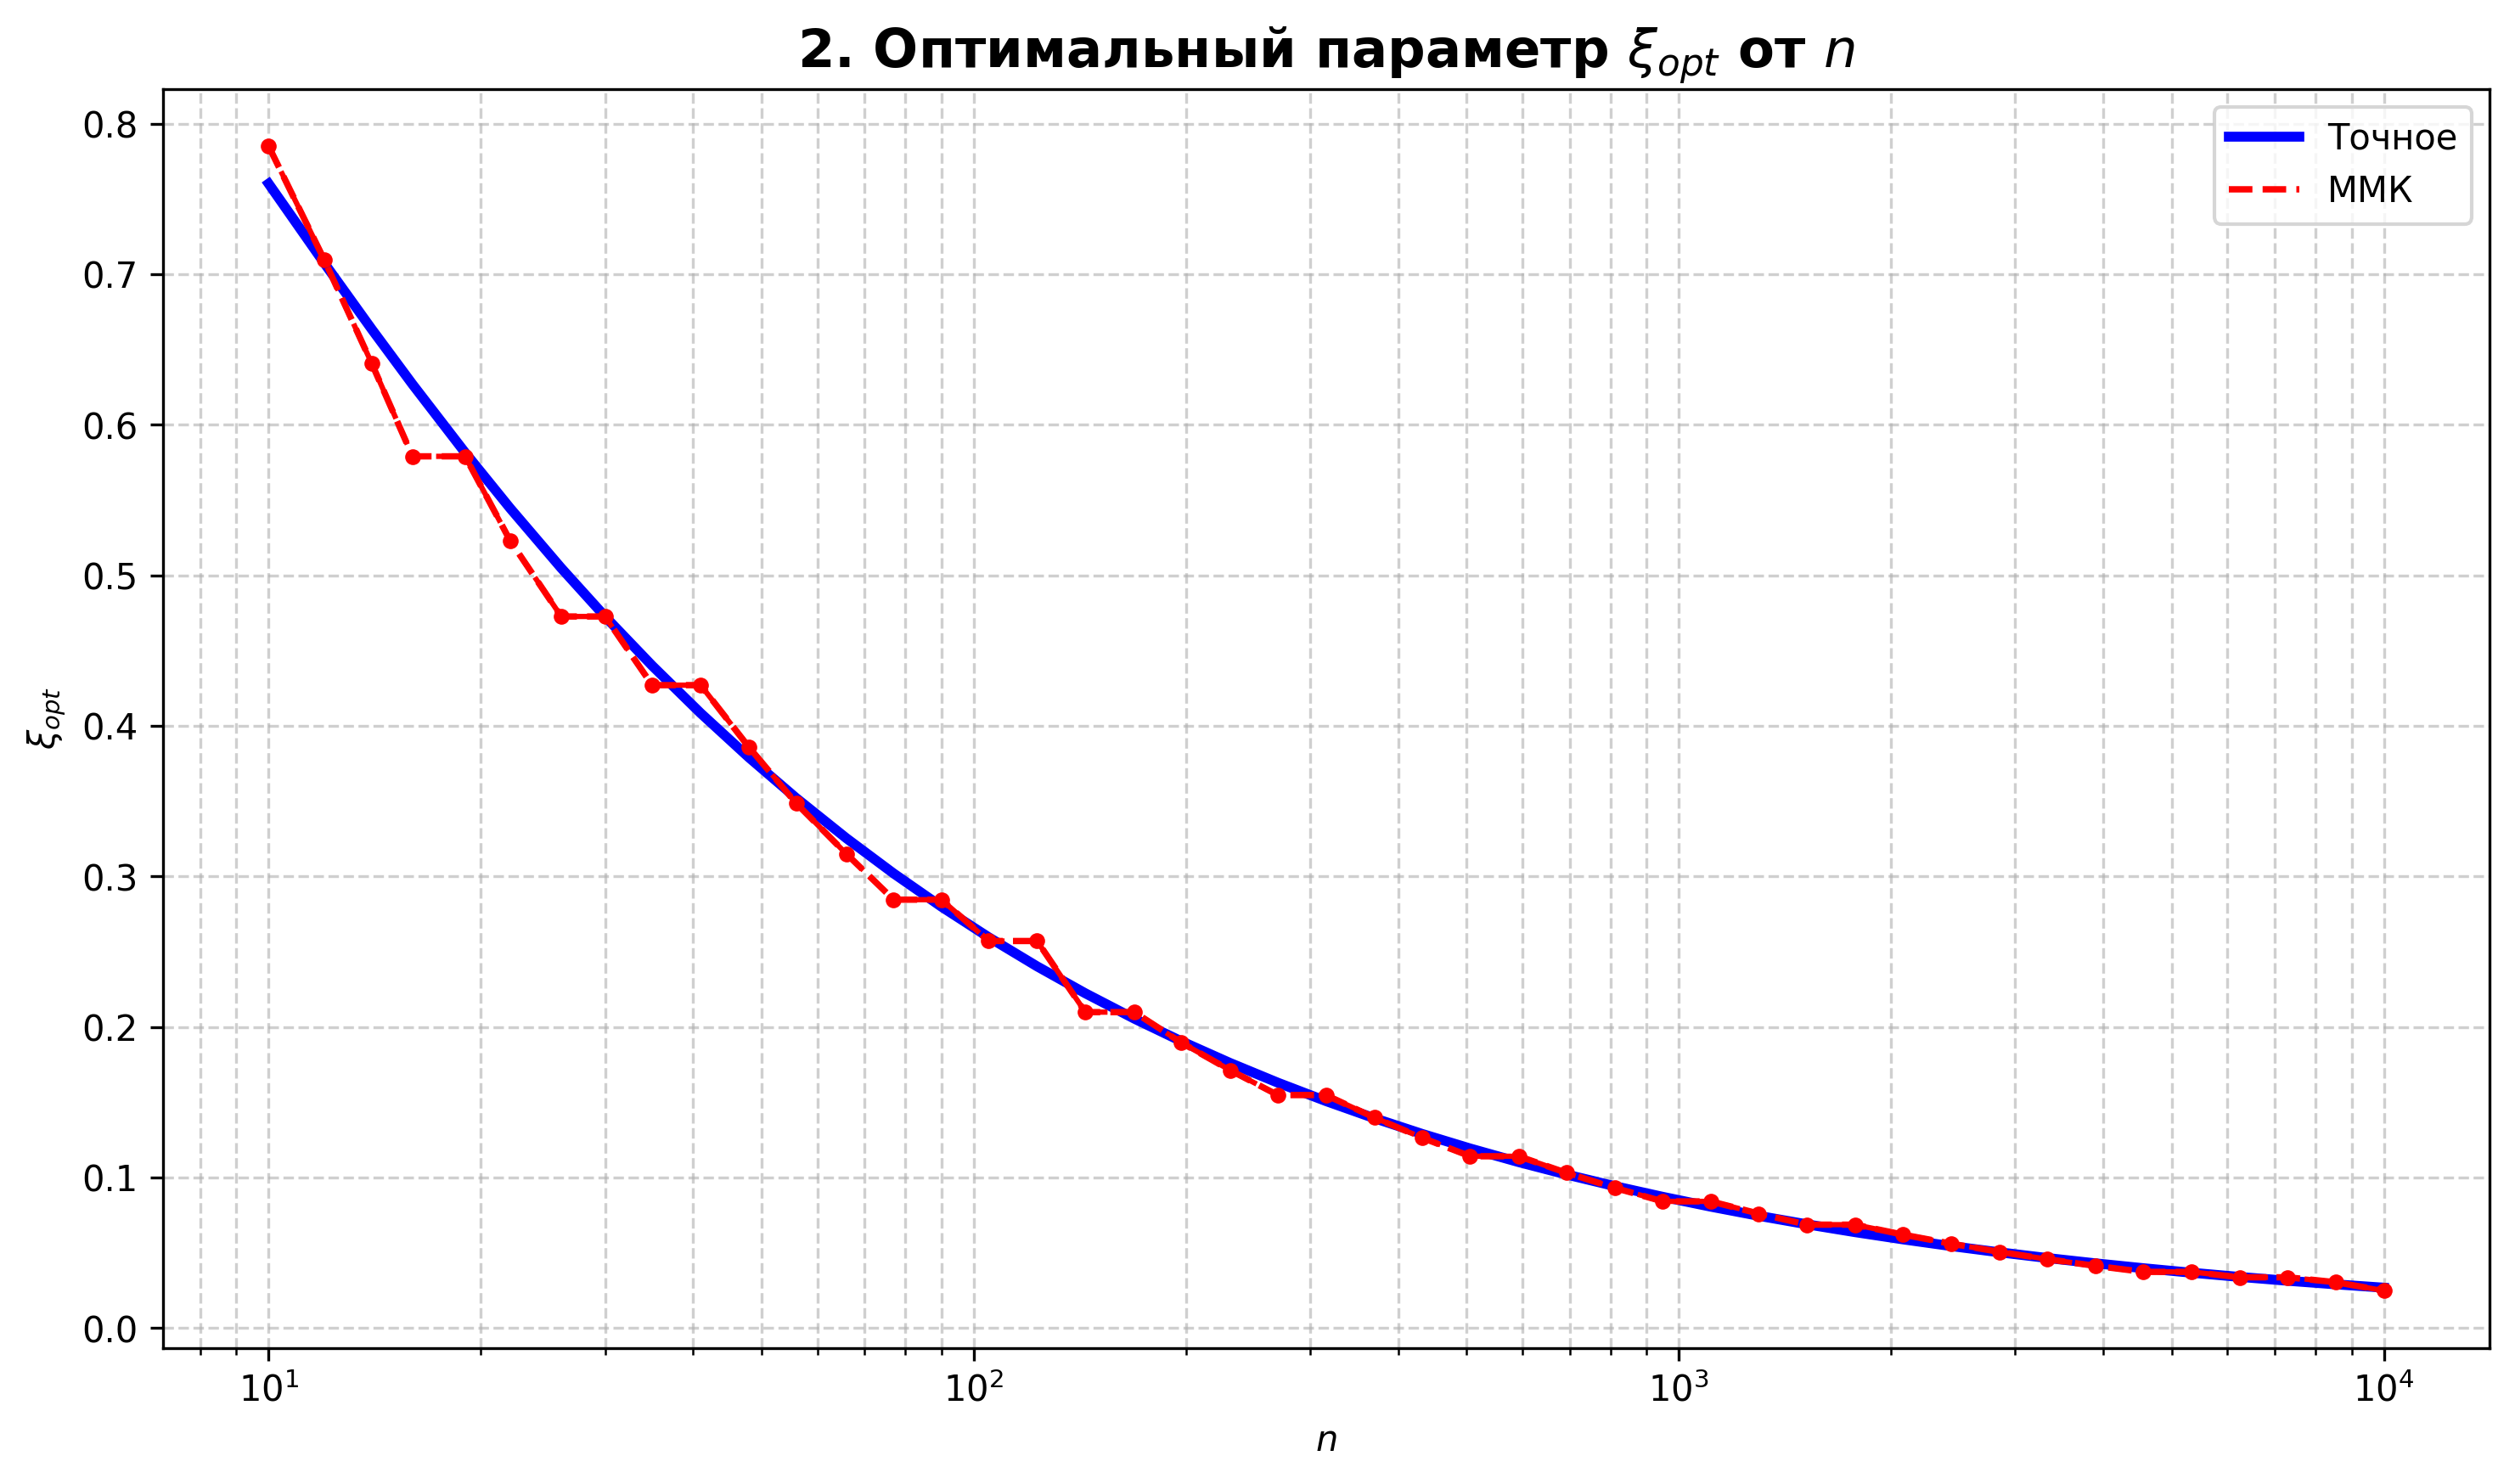
\includegraphics[width=0.85\textwidth]{figures/f13.png}
    \caption{Сравнение точного решения и численного, полученного методом Монте-Карло}
    \label{fig:xi_opt_mmc}
\end{figure}

\newpage

\subsection*{График 3. Зависимость \(\bar{\delta}_{n,\min}\) от объёма выборки \(n\)}

\begin{figure}[ht!]
    \centering
    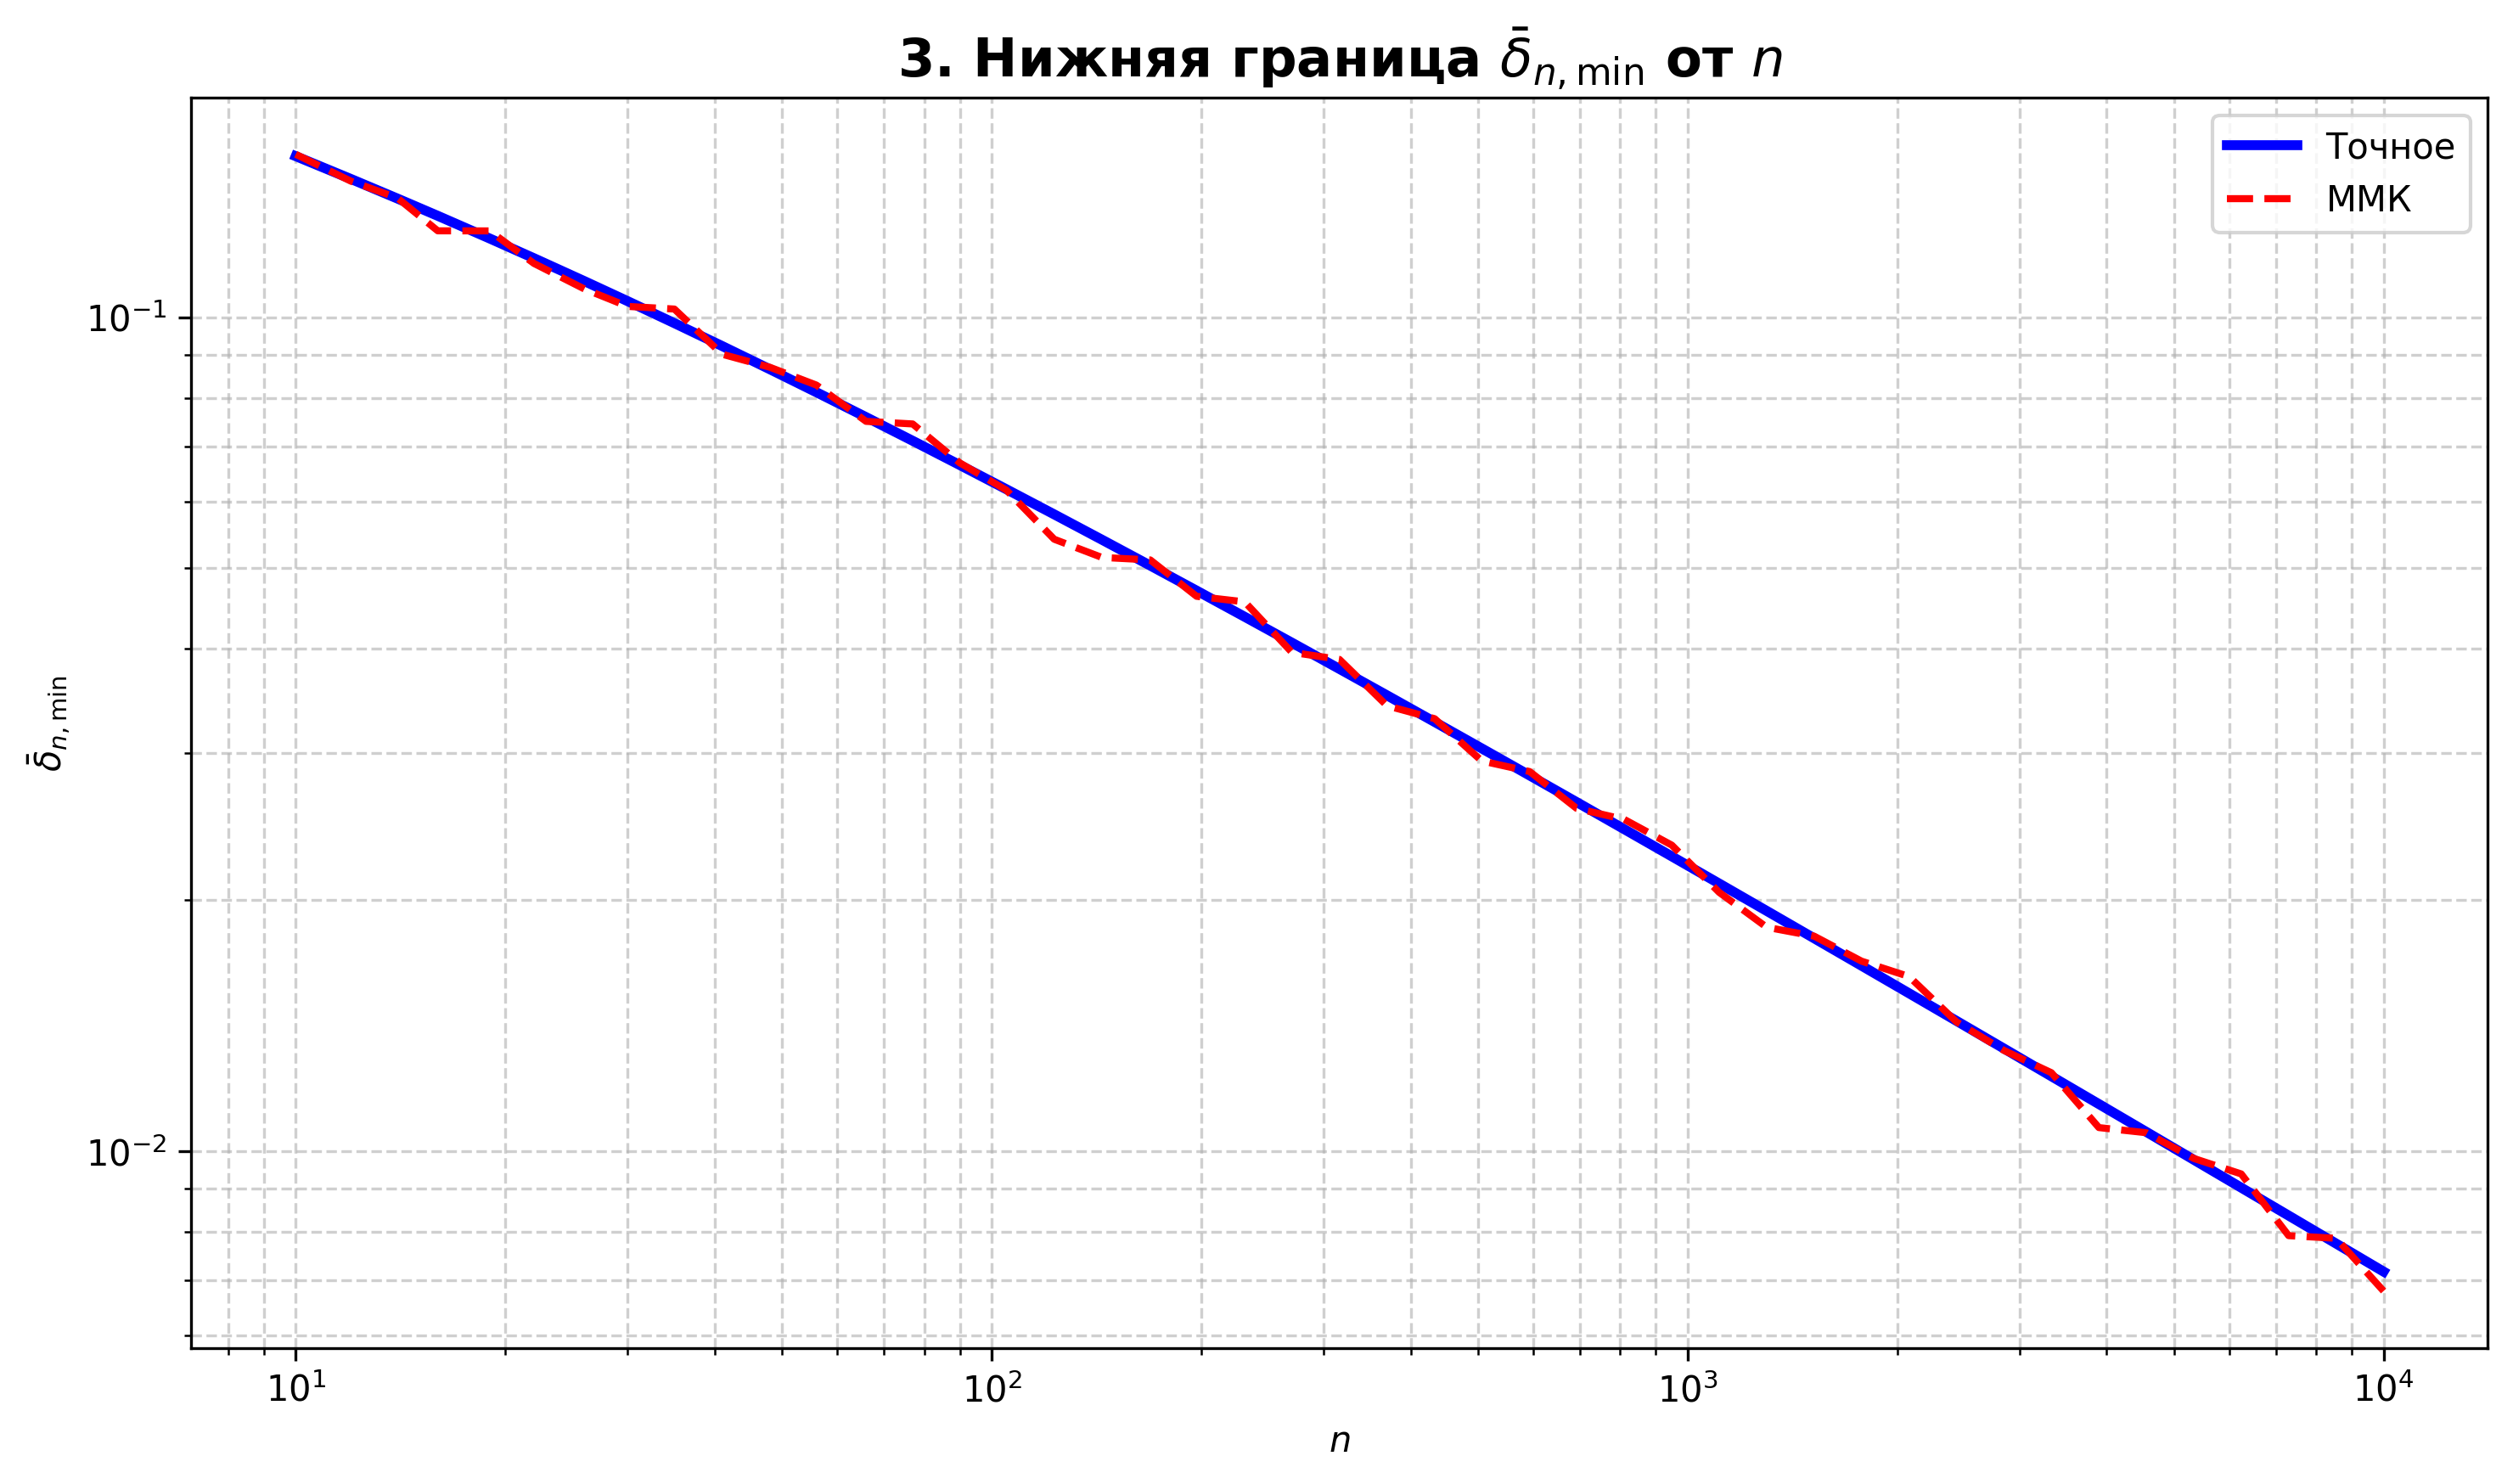
\includegraphics[width=0.85\textwidth]{figures/f14.png}
    \caption{Сравнение точного и численного решений методом Монте-Карло}
    \label{fig:delta_min_mmc}
\end{figure}

\subsection*{График 4. Закон распределения \(\bar{\delta}_{n}(n)\)}

\begin{figure}[ht!]
    \centering
    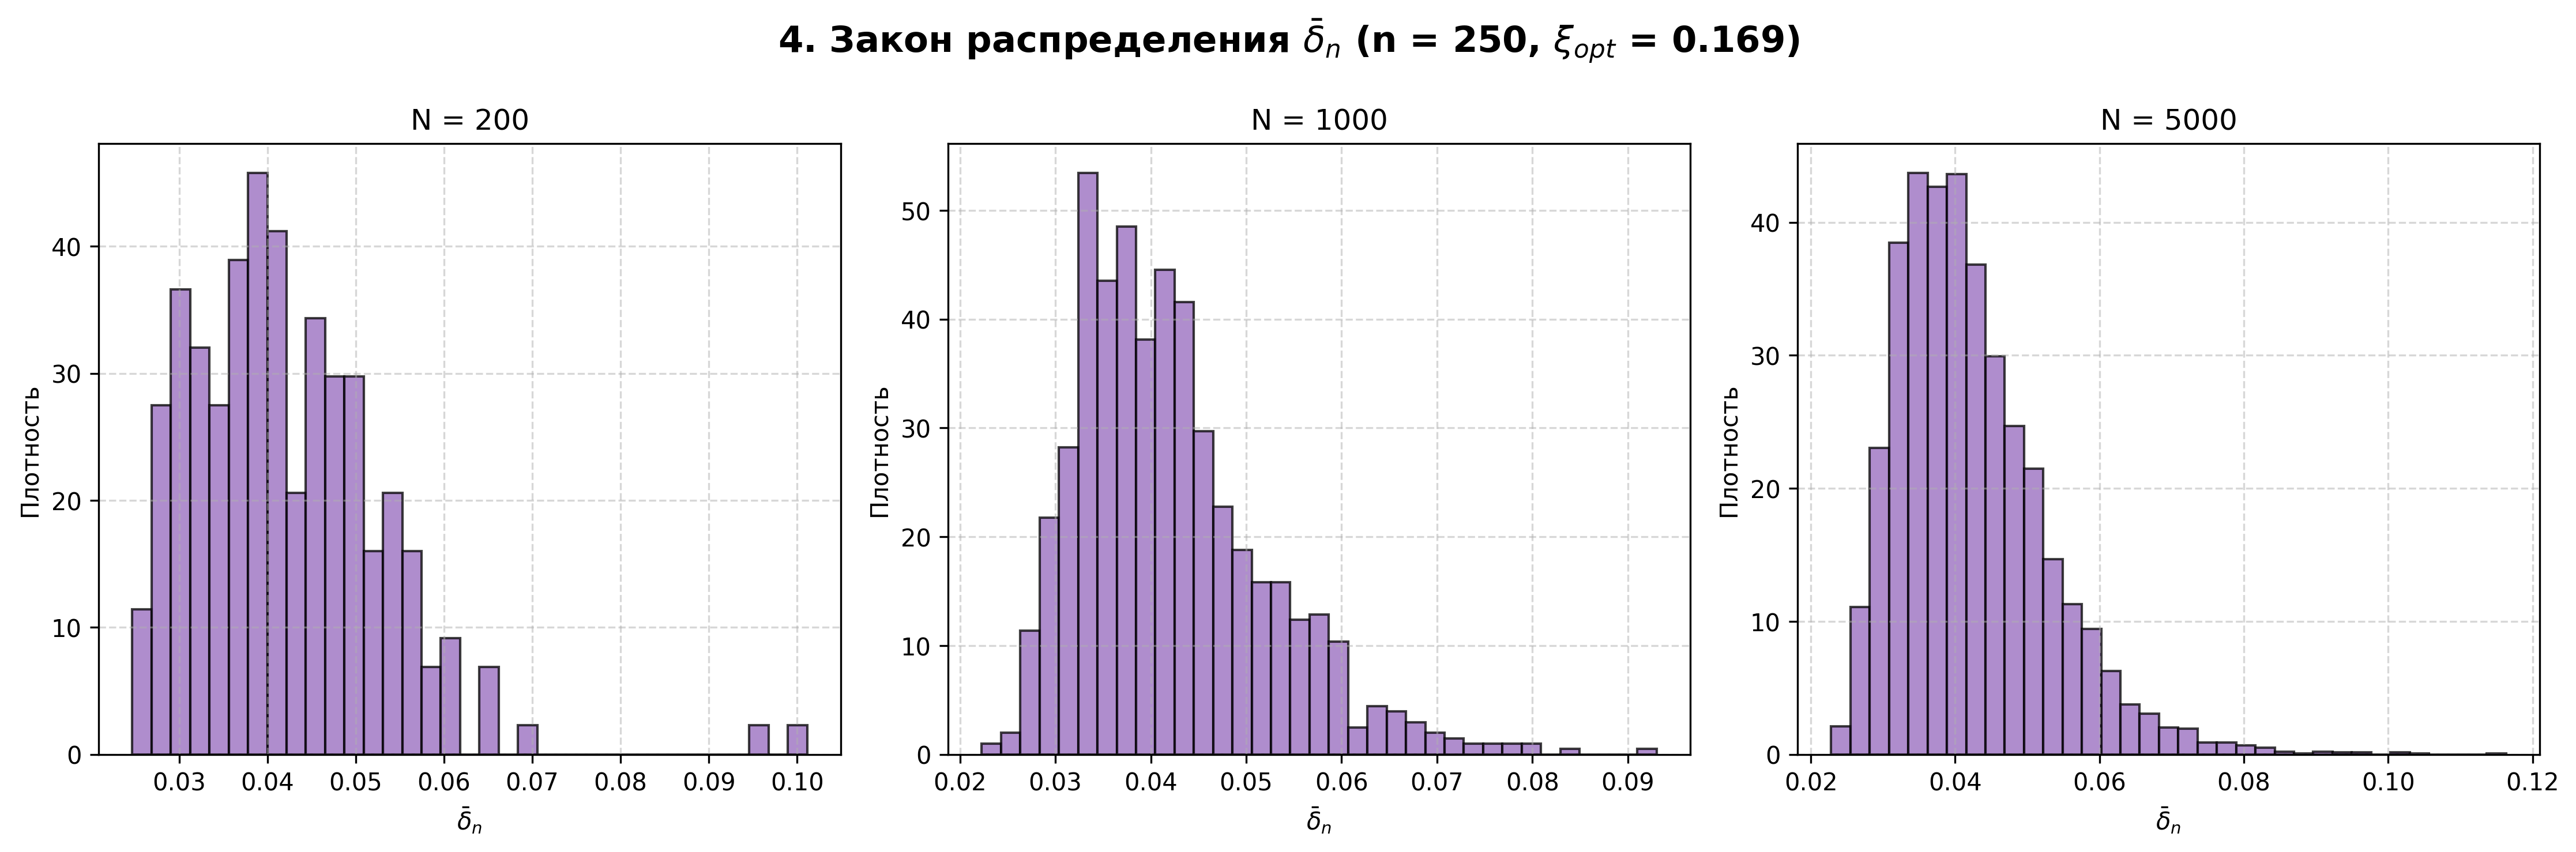
\includegraphics[width=0.95\textwidth]{figures/f15.png}
    \caption{Гистограммы распределения \(\bar{\delta}_n\) ядерной оценки при различных значениях числа повторных реализаций \(N\) (при фиксированном \(n = 250\))}
    \label{fig:delta_distribution}
\end{figure}

\end{document}